\documentclass[10pt]{standalone}
\usepackage{tikz}
\usetikzlibrary{patterns}
\usepackage{pgfplots}
\usepackage{ifthen}
\usetikzlibrary{decorations.markings, calc}




\begin{document}
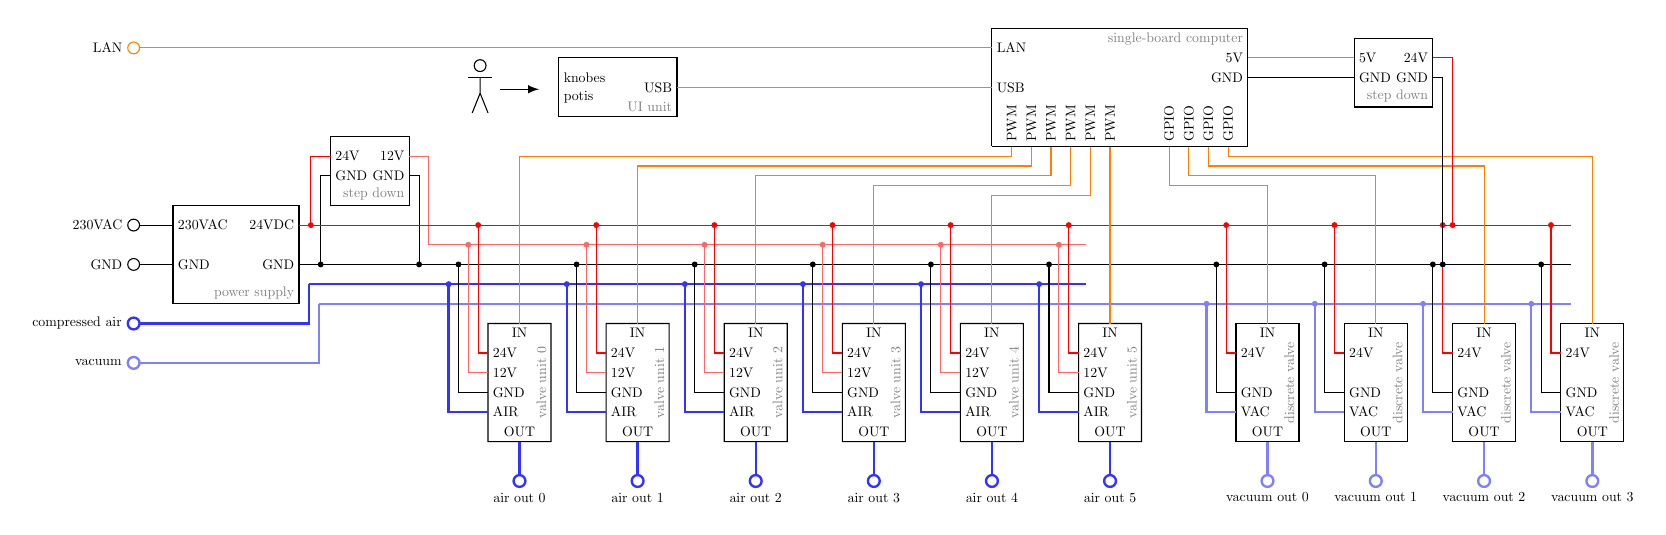
\begin{tikzpicture}[
scale = .5,
connect/.style={circle, fill, inner sep=0pt, minimum height=.75mm},
outerconnect/.style={circle, fill=white, draw, inner sep=0pt, minimum height=1.5mm},
fontnode/.style={scale=.5},
resistor/.style={sloped, scale=.5, fill=white!50, minimum width=1.5cm, draw},
fluid/.style={line width=.3mm, blue!80},
vacuum/.style={line width=.3mm, blue!50},
24v/.style={red},
12v/.style={red!60},
gnd/.style={black},
signal/.style={orange},
]



%% Power Supply
\draw (0,0.5)rectangle++(3.2,-2.5)node[above left, fontnode, gray]{power supply};
\draw (0,0)node[right, fontnode]{230VAC}--++(-1,0)node[outerconnect](PS230){};
\path (PS230.west) node[left, fontnode]{230VAC};
\draw (0,-1)node[right, fontnode]{GND}--++(-1,0)node[outerconnect](PSGND){};
\path (PSGND.west) node[left, fontnode]{GND};

\path (3.2,0)node[left, fontnode]{24VDC}coordinate(24V);
\path (3.2,-1)node[left, fontnode]{GND}coordinate(GND);

%% Step Down Converter
\draw (4,.5) --++ (0,.75)coordinate(ACDCGND)node[right, fontnode]{GND}--++(0,.5)coordinate(ACDC24V)node[right, fontnode]{24V}--++(0,.5)--++(2,0)--++ (0,-.5)coordinate(ACDC12V)node[left, fontnode]{12V}--++ (0,-.5)coordinate(ACDCGNDO)node[left, fontnode]{GND}--++(0,-.75)node[above left, fontnode, gray]{step down} --cycle;
\path (ACDCGND)++(-.25,0)|-(GND)coordinate[midway](x);
\draw[gnd] (ACDCGND)--++(-.25,0)--(x)node[connect]{};
\path (ACDC24V)++(-.5,0)|-(24V)coordinate[midway](x);
\draw[24v] (ACDC24V)--++(-.5,0)--(x)node[connect]{};
\path (ACDCGNDO)++(.25,0)|-(GND)coordinate[midway](x);
\draw[gnd] (ACDCGNDO)--++(.25,0)--(x)node[connect]{};
\path (GND)--(24V)coordinate[midway](xx);
\path (ACDC12V)++(.5,0)|-(xx)coordinate[midway](12V);
\draw[12v] (ACDC12V)--++(.5,0)--(12V);


%% Fluidic
\path (GND)++(.25,-.5)coordinate(AIR);
\draw[fluid] (-1,-2.5)node[outerconnect](C){}-|(AIR);
\path (C.west)node[left, fontnode]{compressed air};
\path (AIR)++(.25,-.5)coordinate(VAC);
\draw[vacuum] (-1,-3.5)node[outerconnect](C){}-|(VAC);
\path (C.west)node[left, fontnode]{vacuum};

%%% Lines
\def\l{20}
\def\ll{32.3} % extra long (gnd, 24v, vacuum)
\draw[gnd] (GND)--++(\ll,0);
\draw[24v] (24V)--++(\ll,0);
\draw[12v] (12V)--++(\l-3.3,0);
\draw[fluid] (AIR)--++(\l-.25,0);
\draw[vacuum] (VAC)--++(\ll-.5,0);


%%% Valve Units
\def\dx{3}
\foreach \i in {0,1,...,5}{
\pgfmathsetmacro{\x}{8+\i*\dx}
\draw (\x,-2.5)coordinate(X)--++(0,-.75)coordinate(24IN)node[right, fontnode]{24V}--++(0,-.5)coordinate(12IN)node[right, fontnode]{12V}--++(0,-.5)coordinate(GNDIN)node[right, fontnode]{GND}--++(0,-.5)coordinate(AIRIN)node[right, fontnode]{AIR}--++(0,-.75)--++(.8,0)coordinate(PVOUT\i)node[above, fontnode]{OUT}--++(.8,0)--++(0,3)node[midway, sloped, above, fontnode, gray]{valve unit \i}--cycle;
\path (X)--++(1.6,0)coordinate[pos=.5](PVIN\i)node[pos=.5,below, fontnode]{IN};

\path (24IN)++(-.25,0)|-(24V)coordinate[midway](x);
\draw[24v] (24IN)--++(-.25,0)--(x)node[connect]{};
\path (12IN)++(-.5,0)|-(12V)coordinate[midway](x);
\draw[12v] (12IN)--++(-.5,0)--(x)node[connect]{};
\path (GNDIN)++(-.75,0)|-(GND)coordinate[midway](x);
\draw[gnd] (GNDIN)--++(-.75,0)--(x)node[connect]{};
\path (AIRIN)++(-1,0)|-(AIR)coordinate[midway](x);
\draw[fluid] (AIRIN)--++(-1,0)--(x)node[connect]{};

\draw[fluid] (PVOUT\i)--++(0,-1)node[outerconnect](x){};
\path (x.south)node[below, fontnode]{air out \i};
}



%%% Discrete Valves
\def\dx{2.75}
\foreach \i in {0,1,...,3}{
\pgfmathsetmacro{\x}{27+\i*\dx}
\draw (\x,-2.5)coordinate(X)--++(0,-.75)coordinate(24IN)node[right, fontnode]{24V}--++(0,-1)coordinate(GNDIN)node[right, fontnode]{GND}--++(0,-.5)coordinate(VACIN)node[right, fontnode]{VAC}--++(0,-.75)--++(.8,0)coordinate(DVOUT\i)node[above, fontnode]{OUT}--++(.8,0)--++(0,3)node[midway, sloped, above, fontnode, gray]{discrete valve}--cycle;
\path (X)--++(1.6,0)coordinate[pos=.5](DVIN\i)node[pos=.5,below, fontnode]{IN};

\path (24IN)++(-.25,0)|-(24V)coordinate[midway](x);
\draw[24v] (24IN)--++(-.25,0)--(x)node[connect]{};
\path (GNDIN)++(-.5,0)|-(GND)coordinate[midway](x);
\draw[gnd] (GNDIN)--++(-.5,0)--(x)node[connect]{};
\path (VACIN)++(-.75,0)|-(VAC)coordinate[midway](x);
\draw[vacuum] (VACIN)--++(-.75,0)--(x)node[connect]{};

\draw[vacuum] (DVOUT\i)--++(0,-1)node[outerconnect](x){};
\path (x.south)node[below, fontnode]{vacuum out \i};
}



%%% BBB
\path (21.3, 2)coordinate(BBBPWM);
\path (25.3, 2)coordinate(BBBGPIO);


\foreach \i in {0,1,...,5}{
\pgfmathsetmacro{\dy}{.25 + \i*.25}
\pgfmathsetmacro{\dx}{\i*.5}
\draw[signal] (BBBPWM)++(\dx, 0)node[right,rotate=90, fontnode, black]{PWM}--++(0,-\dy)-|(PVIN\i);
}

\foreach \i in {0,1,...,3}{
\pgfmathsetmacro{\dy}{1 - \i*.25}
\pgfmathsetmacro{\dx}{\i*.5}
\draw[signal] (BBBGPIO)++(\dx, 0)node[right,rotate=90, fontnode, black]{GPIO}--++(0,-\dy)-|(DVIN\i);
}

\draw (BBBPWM)++(-.5,0)--++(6.5,0)--++(0,1.75)coordinate(BBBGND)node[left,fontnode]{GND}--++(0,.5)coordinate(BBB5V)node[left,fontnode]{5V} --++ (0,.75)node[fontnode, gray, below left]{single-board computer}--++(-6.5,0)--++(0,-.5)coordinate(BBBLAN)node[right, fontnode]{LAN}--++(0,-1)coordinate(BBBUSB)node[right, fontnode]{USB}--++(0,-1.5);



%% Step Down Converter
\draw (BBBGND)++(2.7,-.75) --++ (0,.75)coordinate(ACDCGND)node[right, fontnode]{GND}--++(0,.5)coordinate(ACDC5V)node[right, fontnode]{5V}--++(0,.5)--++(2,0)--++ (0,-.5)coordinate(ACDC24V)node[left, fontnode]{24V}--++ (0,-.5)coordinate(ACDCGNDO)node[left, fontnode]{GND}--++(0,-.75)node[above left, fontnode, gray]{step down} --cycle;
\draw[gnd] (ACDCGND)--(BBBGND);
\path (ACDC24V)++(.5,0)|-(24V)coordinate[midway](x);
\draw[24v] (ACDC24V)--++(.5,0)--(x)node[connect]{};
\path (ACDCGNDO)++(.25,0)|-(GND)coordinate[midway](x);
\draw[gnd] (ACDCGNDO)--++(.25,0)--(x)node[connect]{};
\draw[12v] (ACDC5V)--(BBB5V);


%% UI
\draw (BBBUSB)++(-8,0)coordinate(UIUSB)node[left, fontnode]{USB}--++(0,-.75)node[above left, fontnode, gray]{UI unit}--++(-3,0)--++(0,.5)coordinate(potis)node[right, fontnode]{potis}--++(0,.5)coordinate(knobes)node[right, fontnode]{knobes}--++(0,.5)--++(3,0)--++(0,-.75);
\draw[signal] (UIUSB)--(BBBUSB);

\path (potis)++(-2,.5)coordinate(user);
\draw (user)++(0,.3)circle(.15);
\draw (user)++(-.3,0)--++(.6,0);
\draw (user)--++(0,-.4)--++(-.2,-.5);
\draw (user)++(0,-.4)--++(.2,-.5);

\draw[-latex] (user)++(.5,-.3)--++(1,0);

%% LAN
\path (BBBLAN)-| (PS230) coordinate[midway](x);
\draw[signal] (BBBLAN)--(x)node[outerconnect](LAN){};
\path (LAN.west)node[left, fontnode]{LAN};

\end{tikzpicture}
\end{document}